\hypertarget{chap2}{%
\chapter{De tussenpersoon verwijderen}\label{chap2}}

In het vorige hoofdstuk hebben we besproken dat bitcoin een peer-to-peer systeem is voor de overdracht van waarde. Voordat we ingaan op hoe dat werkt, kijken we eerst hoe een traditionele bank of betalingsverwerker omgaat met het beheer van eigendom en overdrachten van activa.

\section{Banken zijn slechts grootboeken}

Hoe werkt een digitale betaling via de bank, \textit{PayPal} of \textit{ApplePay}? Heel eenvoudig, fungeren deze tussenpersonen als veredelde grootboeken van rekeningen en overschrijvingen.

De functie van een bank is traditioneel gezien het opslaan en beschermen van tegoeden. In de huidige tijd zijn die tegoeden echter vooral elektronisch, in plaats van fysiek in de vorm van munten of bankbiljetten. Daarom is het beheer en de bescherming van data nu een belangrijke taak van een bank. Aangezien de data elektronisch zijn, is de beveiliging daarvan ook voornamelijk digitaal. Banken zetten softwarematige inbraakdetectiesystemen in, creëren back-ups om tegen dataverlies te beschermen, ondergaan audits van derden om te waarborgen dat hun interne processen intact blijven en sluiten preventief verzekeringen af voor het geval dat er iets mis mocht gaan.

\clearpage

Hieronder zie je hoe banken werken. In dit voorbeeld hebben we het over een bank, maar je kan dit lezen als elke partij die betalingen verwerkt. We beginnen met een grootboek van rekeningen waaruit blijkt dat Alice en Bob geld hebben gestort bij de bank.

\begin{alltt}
\underline{Grootboek van de bank}

    1. Alice: Credit voor cash storting +2€
    2. Bob: Credit voor cash storting +10€
\end{alltt}

Als Alice €2 naar Bob wil overmaken, neemt ze contact op met haar bank of gebruikt ze de website of mobiele app van haar bank. Ze logt vervolgens in bij de bank met haar gebruikersnaam en wachtwoord of pincode, waarna ze de overboeking aanvraagt. Deze transactie wordt door de bank geregistreerd in hun grootboek.

\begin{alltt}
\underline{Grootboek van de bank}

    1. Alice: Credit voor cash storting +€2
    2. Bob: Credit voor cash storting +10€
    3. Alice: Debet -2€
    4. Bob: Credit +2€
\end{alltt}

De bank heeft de credits en debets en de bijbehorende saldi geregistreerd. Het geld is nu overgemaakt.

\section{Het probleem van dubbele uitgaven}

Wat gebeurt er als Alice diezelfde twee dollar nu weer probeert uit te geven? Dit wordt het \textit{dubbele-uitgavenprobleem} genoemd. Zij dient het verzoek in bij de bank, maar de bank zegt: "Sorry, we zien dat je die €2 al hebt uitgegeven aan Bob. Je kan dat geld niet meer uitgeven."

Als je te maken hebt met een centrale autoriteit, zoals een bank, kan deze gemakkelijk opmerken wanneer je probeert geld uit te geven dat je al hebt besteed. Dat is omdat zij de enige zijn die bevoegd zijn om wijzigingen in het grootboek aan te brengen. Ze hebben verschillende interne processen, waaronder back-ups en audits, om te waarborgen dat het grootboek correct is en om manipulatie ervan te voorkomen. We noemen dit een \textit{gecentraliseerd} systeem omdat er sprake is van één enkel controlepunt.

\begin{figure}[h]
    \centering
    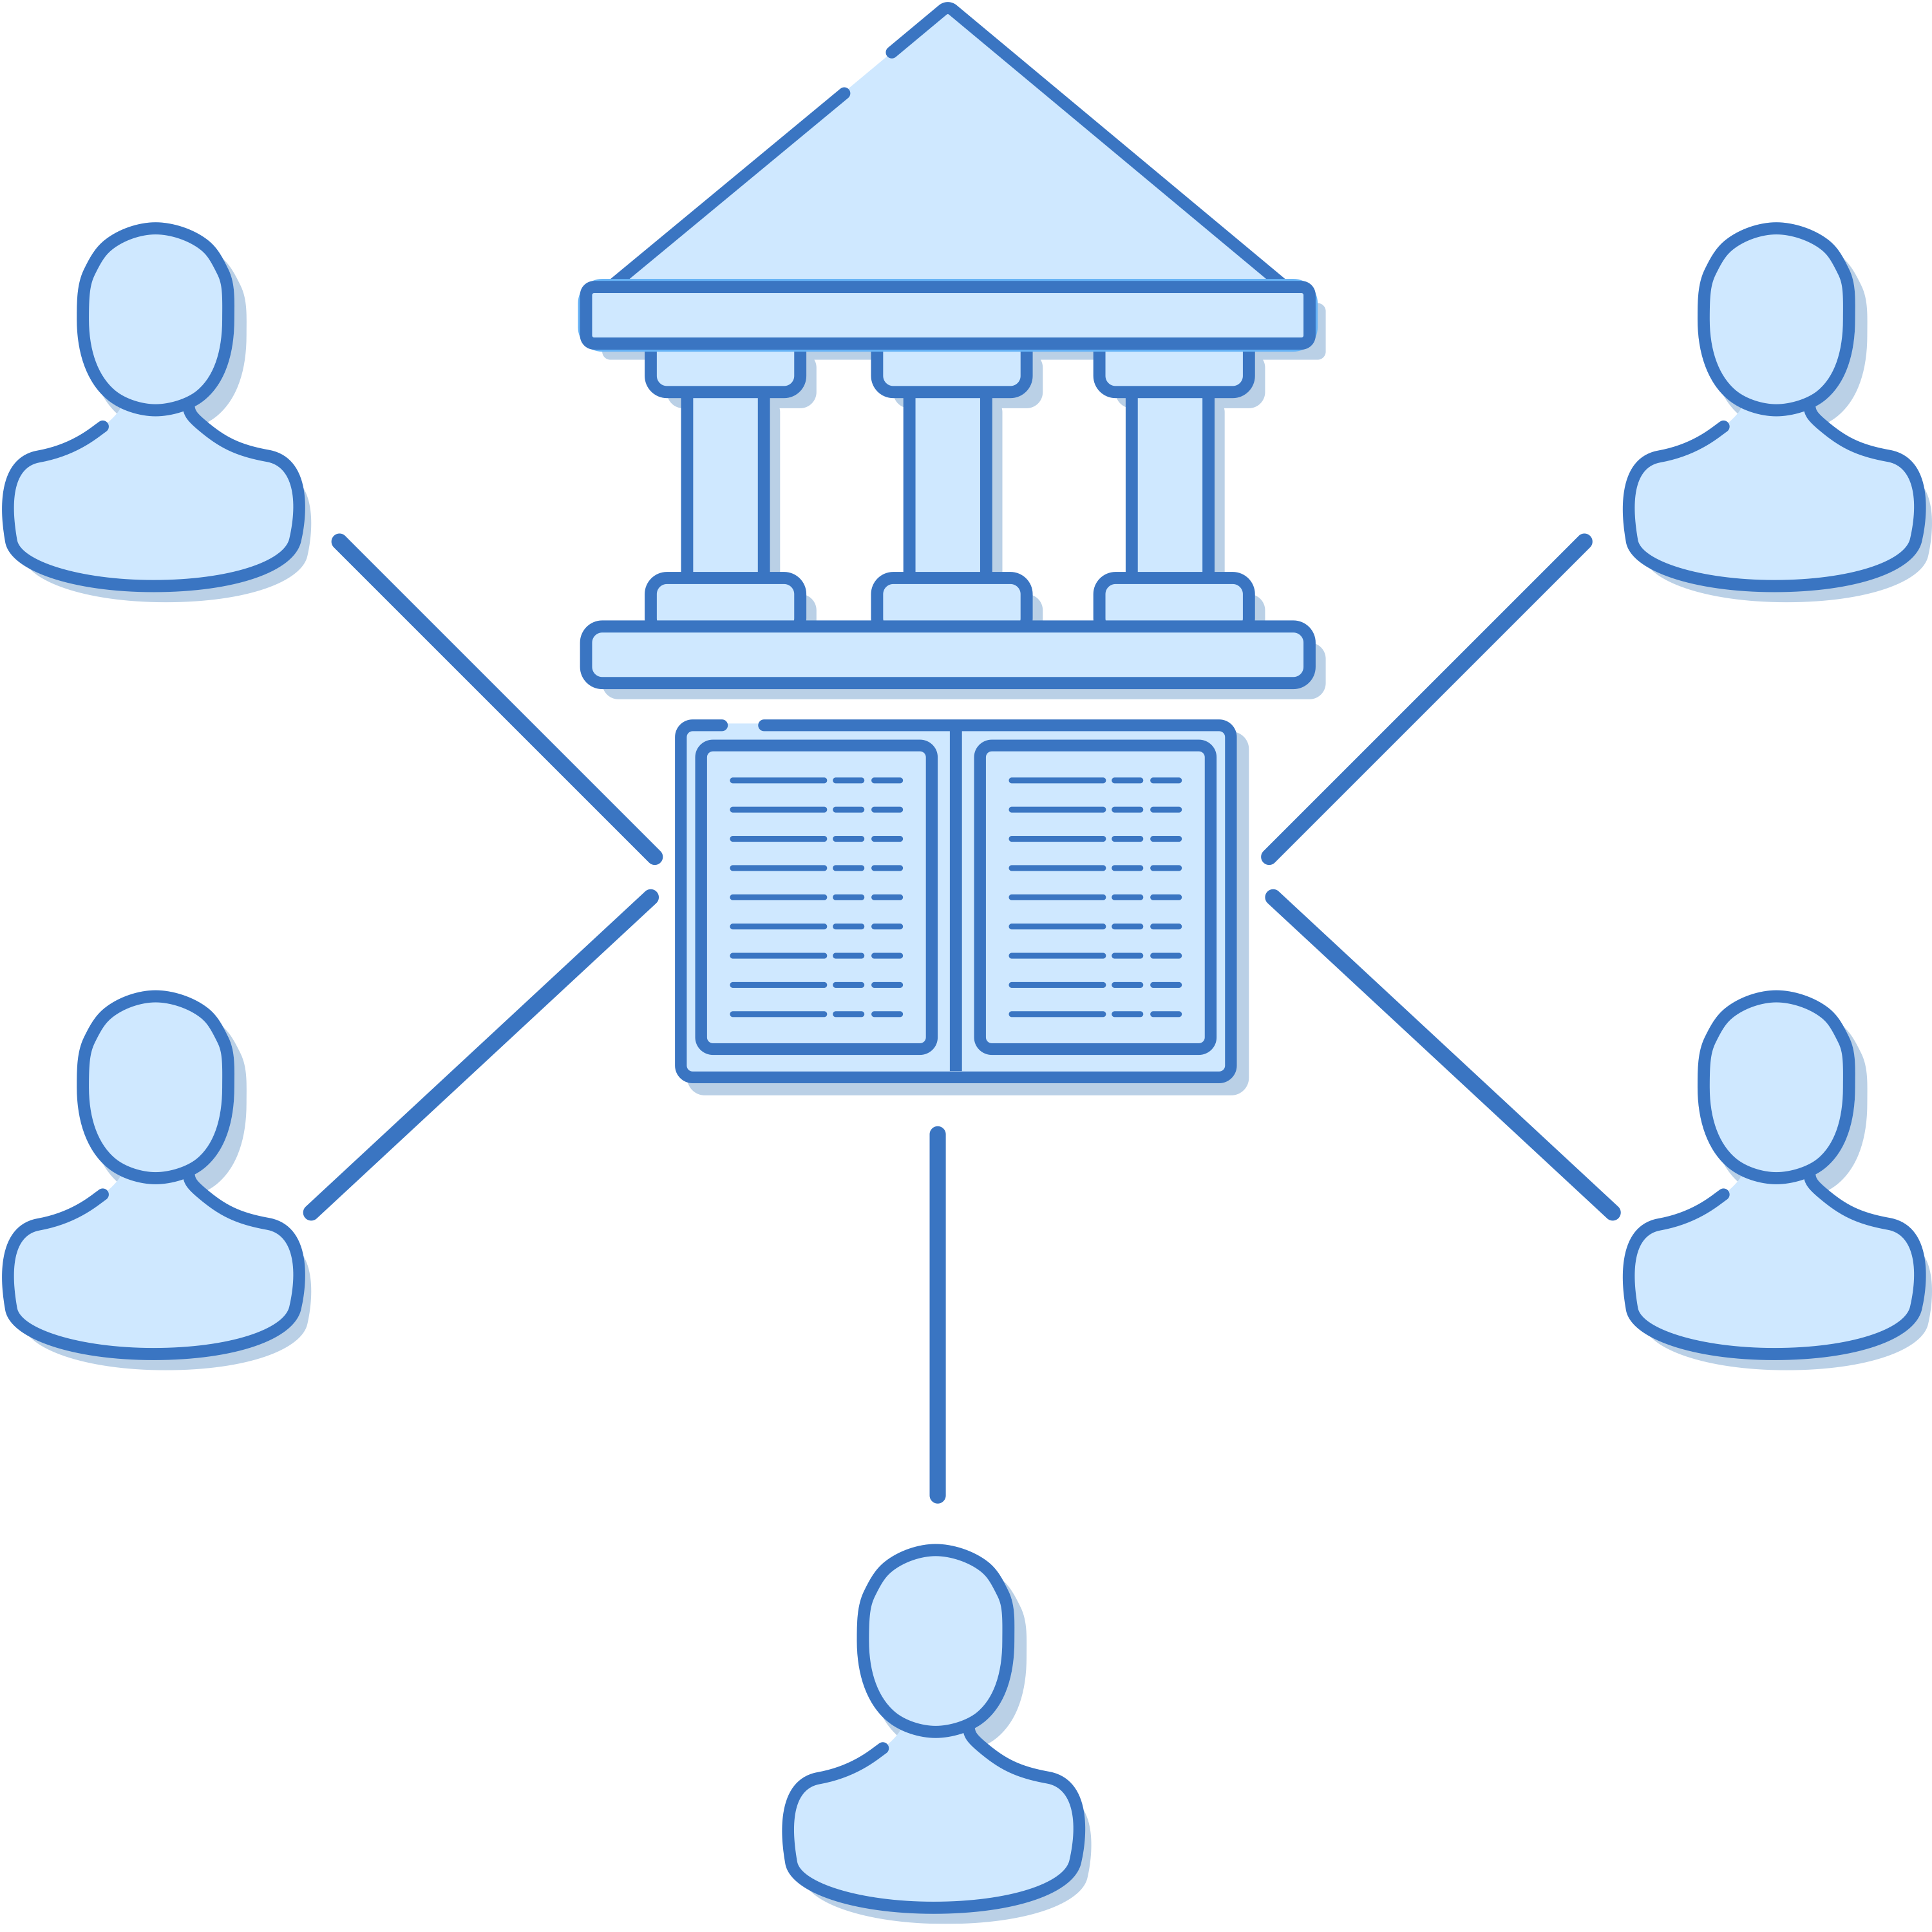
\includegraphics[width=0.6\textwidth]{images/fig2.png}
    \caption{\footnotesize{\textit{De bank houdt een grootboek bij waar iedereen toegang toe heeft, maar alleen via de bank bij kan.}}}
    \label{fig2}
\end{figure}

\section{Het grootboek delen tussen verschillende partijen}

Het eerste probleem dat bitcoin wil aanpakken, is het uitschakelen van een tussenpersoon door een \textit{peer-to-peer} systeem te creëren. Stel je eens voor dat banken er niet meer zijn en we ons financiële systeem vanuit het niets weer moeten opbouwen. Hoe kunnen we een grootboek bijhouden zonder een centrale instantie? Als we geen centraal grootboek hebben, dan moet het grootboek van het volk zijn. Leve de revolutie. Zo pakken we het aan.

Eerst komen een aantal mensen samen en creëren zij een \textit{netwerk}. Dit betekent simpelweg dat een manier bestaat om informatie met elkaar te delen. Laten we zeggen dat we telefoonnummers of Snapchat-accounts uitwisselen. Wanneer Alice geld wil overmaken naar Bob, belt ze niet naar de bank, maar zegt ze tegen al haar vrienden: \textquotedbl{}Ik stuur €2 naar Bob\textquotedbl{}. Iedereen bevestigt met: \textquotedbl{}Top, we noteren het\textquotedbl{}, en schrijft het in hun eigen kopie van het grootboek. Het ziet er uit zoals in Figuur \ref{fig3}.

\begin{figure}[h]
    \centering
    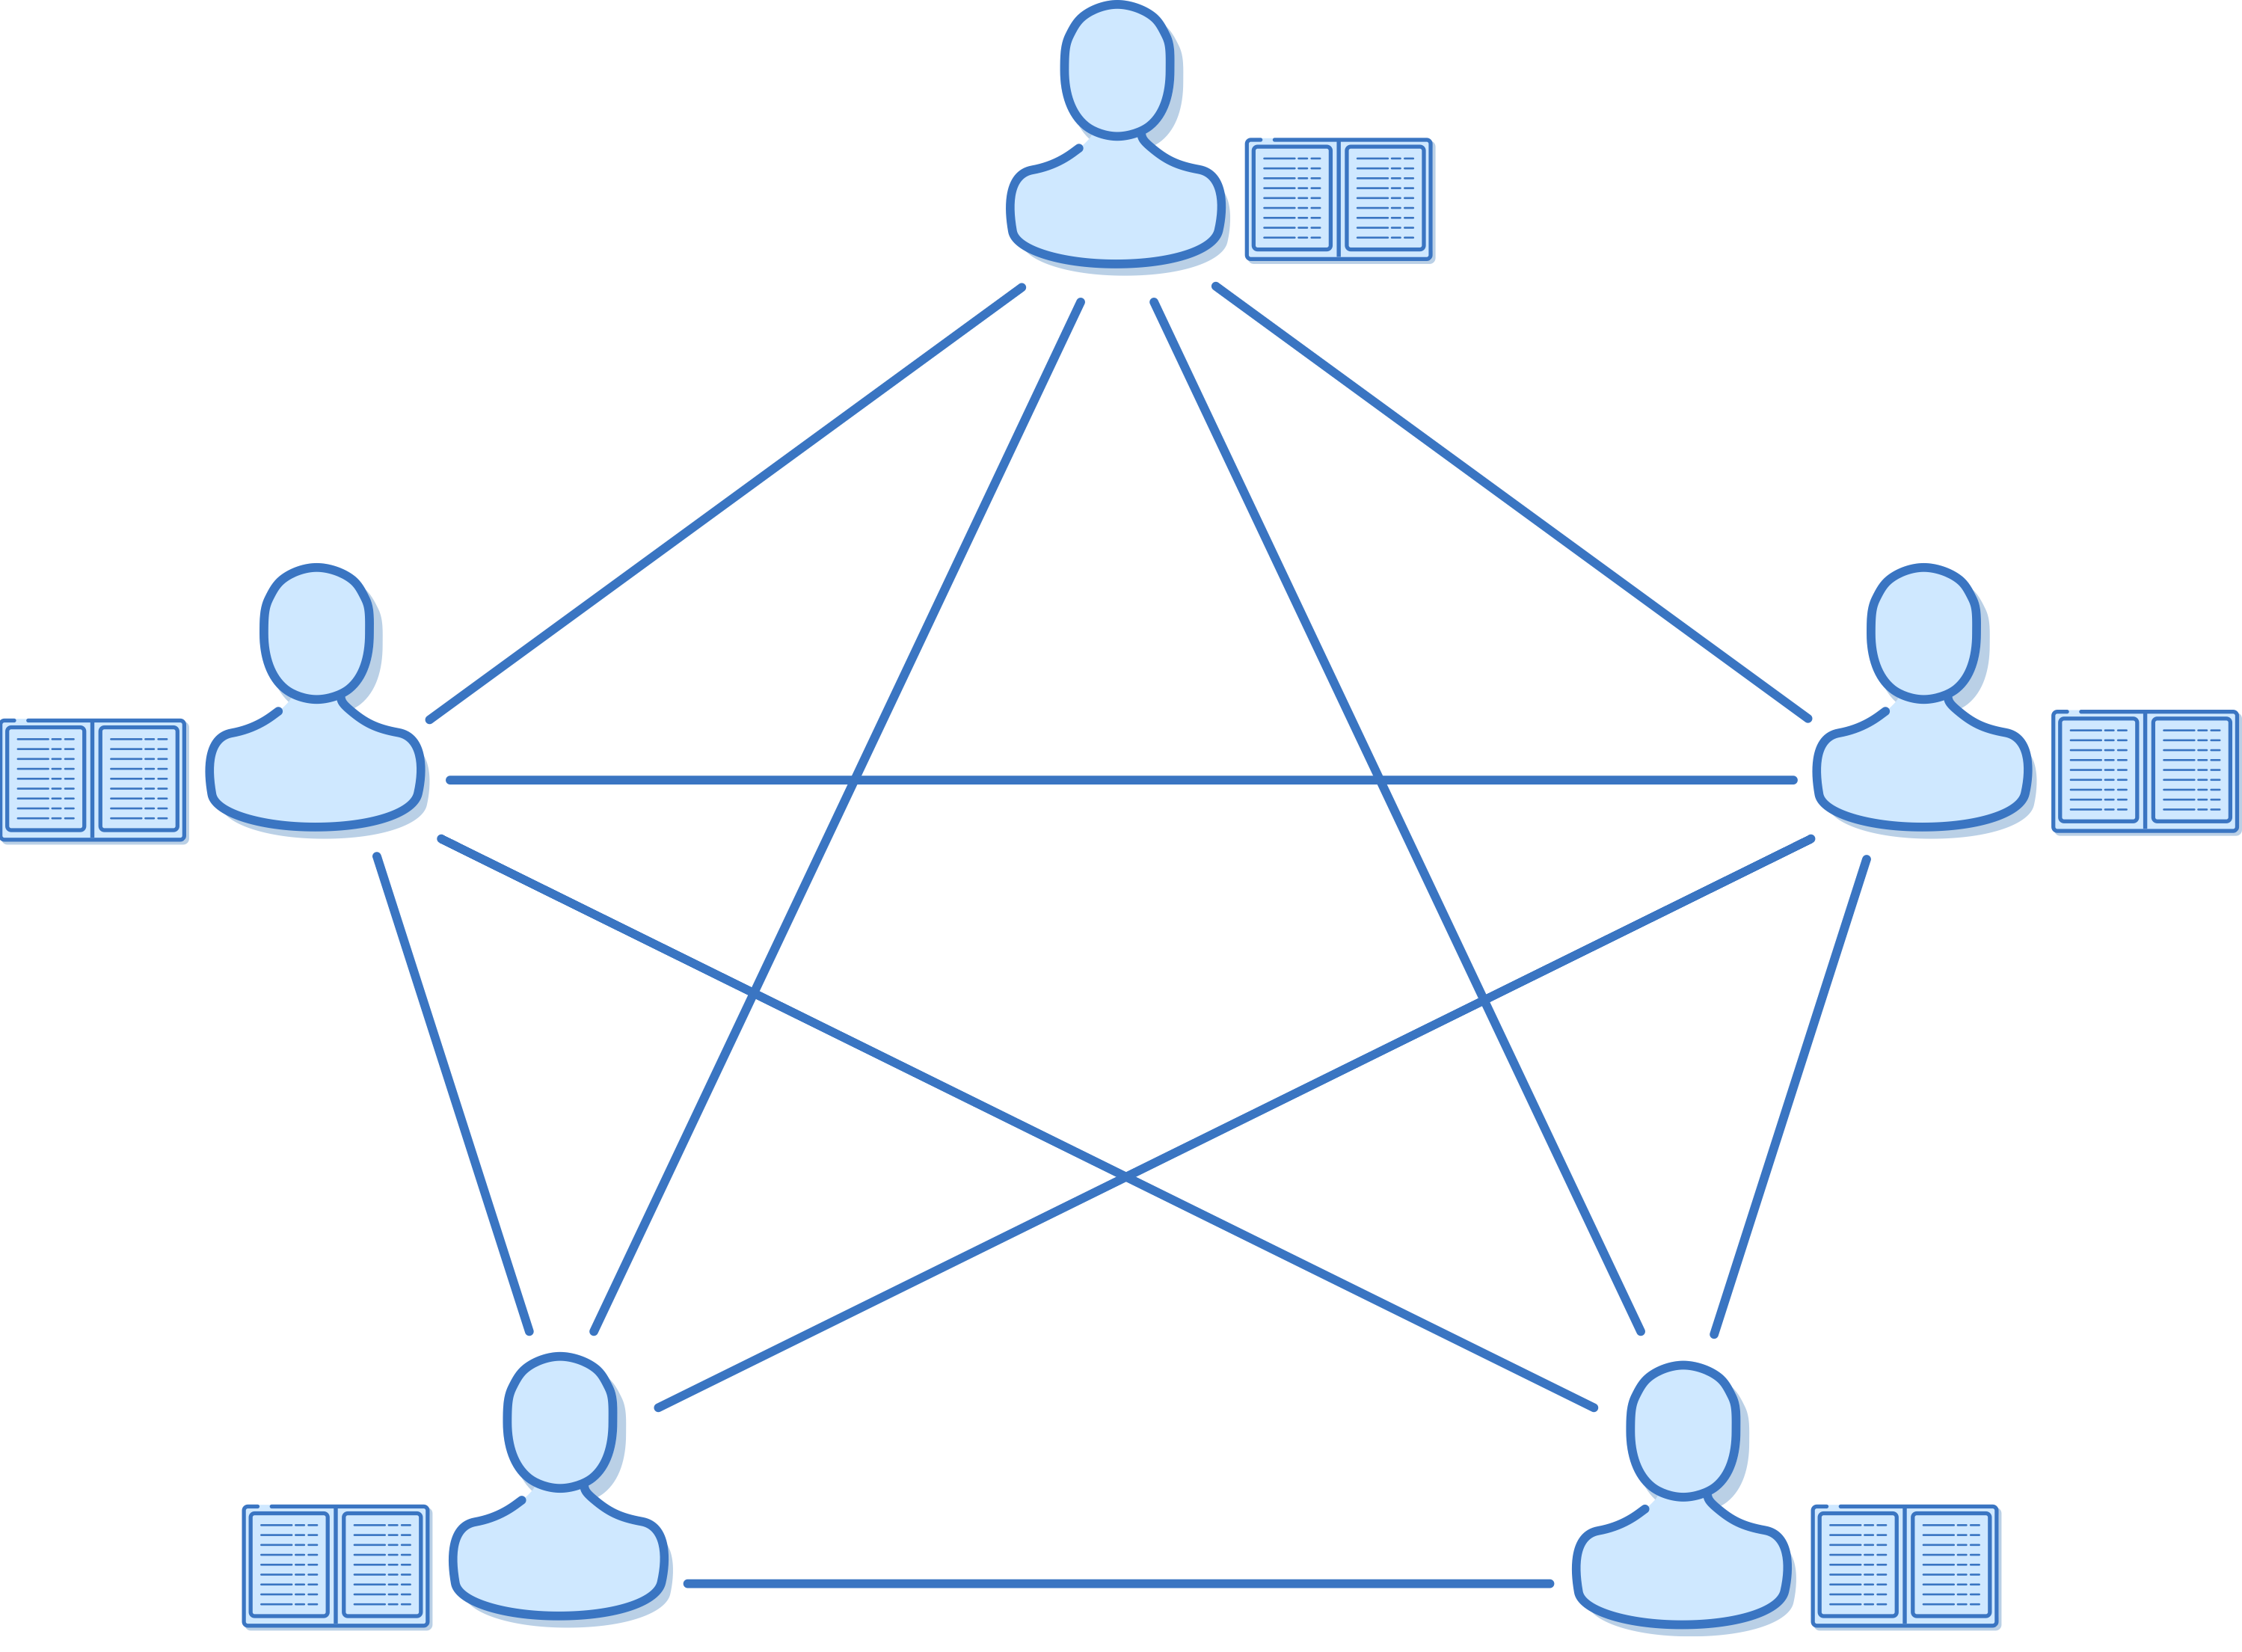
\includegraphics[width=0.6\textwidth]{images/fig3.png}
    \caption{\footnotesize{\textit{Iedereen heeft een eigen kopie van het grootboek, waar ze onafhankelijk van een ander bij kunnen.}}}
    \label{fig3}
\end{figure}

Dus nu beschikt iedereen, en niet alleen de bank, over een kopie van het grootboek. Als iemand geld wil uitgeven, informeren zij al hun vrienden. Iedereen houdt de transacties bij. Het grootboek bevindt zich niet langer op één centrale locatie. Dit wordt \textit{gedistribueerd} genoemd. Het wordt ook wel \textit{decentraal} genoemd, omdat er geen centrale entiteit meer is die de controle heeft. Er is geen tussenpersoon meer nodig waarop je moet kunnen vertrouwen.


Nu we geen bemiddelaar meer hebben, hoe gaan we dan met dubbele uitgaven om? Wie of wat kunnen we aanspreken (in plaats van de bank) om te verifiëren dat het geld dat wordt uitgegeven nog niet eerder is uitgegeven? Aangezien iedereen een kopie van het grootboek bezit, zouden we in feite iedereen moeten raadplegen. Het systeem dat we op dit moment bespreken, berust \textit{op consensus}, omdat er consensus binnen het netwerk bestaat. Iedereen is het eens over één en dezelfde versie van de waarheid.

Als Alice probeert de €2 die ze al naar Bob heeft overgemaakt nog eens uit te geven, dan zal iedereen op het netwerk haar transactie afwijzen. De leden van het netwerk zullen hun grootboeken controleren en Alice mededelen dat het geld reeds is uitgegeven. Ze zullen haar tweede transactie met dezelfde €2 dus niet registreren. We hebben nu een peer-to-peer consensusnetwerk voor het registreren van eigendom en overdracht van tegoeden.

Zolang partijen \textit{toestemming} nodig hebben om aan ons gedistribueerde grootboek deel te nemen, en we erop kunnen \textit{vertrouwen} dat elke partij eerlijk handelt, werkt het systeem goed. Echter, dit soort systemen kunnen niet opgeschaald worden voor gebruik door miljoenen mensen over de hele wereld. Gedistribueerde systemen die bestaan uit willekeurige deelnemers zijn van nature onbetrouwbaar. Er zijn bijvoorbeeld mensen die zo nu en dan offline zijn. Dit betekent dat ze mogelijk niet op de hoogte zijn van onze transacties op het moment dat we die doorvoeren. Sommigen zouden ons zelfs actief kunnen proberen te bedriegen, door te beweren dat bepaalde transacties wel of niet hebben plaatsgevonden. Daarnaast kunnen er nieuwe mensen aan het netwerk deelnemen, waardoor er conflicterende versies van het grootboek kunnen ontstaan.

In het volgende deel onderzoeken we hoe iemand zou kunnen proberen om vals te spelen.

\section{De dubbele-uitgaven aanval}

Als ik Alice ben, kan ik \textit{samenspannen} met een aantal van de andere mensen en hen vertellen: \textquotedbl{}Als ik geld uitgeef, schrijf het dan niet in jullie grootboek. Doe alsof het nooit gebeurd is.\textquotedbl{} Laten we eens kijken hoe Alice zo'n dubbele-uitgaven aanval kan uitvoeren.

Beginnend met een saldo van €2, doet Alice het volgende:

\begin{enumerate}
    \item Ze stuurt haar €2 naar Bob, om een reep chocolade te kopen. Nu heeft Alice €0 over.
    \item David, Eva en Femke spannen samen met Alice en schrijven de transactie van Alice naar Bob niet in hun grootboeken. In hun exemplaar heeft Alice haar geld nooit uitgegeven en heeft ze nog steeds een saldo van €2.
    \item Charlotte is een eerlijke grootboekhouder. Ze registreert correct de transactie van Alice naar Bob. In haar grootboek heeft Alice €0.
    \item Henri was een week op vakantie en heeft nog nooit van de transactie gehoord. Hij sluit zich aan bij het netwerk en vraagt om een kopie van het grootboek.
    \item Henri krijgt 4 valse kopieën (David, Eva, Femke en Alice) en één eerlijke kopie (Charlotte). Hoe bepaalt hij welke echt is? Zonder beter systeem vertrouwt hij de meerderheid van deelnemers en wordt dus misleidt. Hij neemt aan dat het nep-grootboek klopt.
    \item Alice koopt een chocoladereep van Henri met de €2 die ze eigenlijk niet heeft. Henri accepteert het omdat voor zo ver hij weet, Alice nog steeds €2 op haar rekening heeft.
    \item Alice heeft nu 2 chocoladerepen en er is €4 aan nepgeld gemaakt in het systeem. Ze betaalt haar vrienden met chocoladerepen, en ze herhalen de aanval 100 keer op elke nieuwe persoon die lid wordt van het netwerk.
    \item Alice heeft nu alle chocoladerepen en alle anderen hebben grote zakken nepgeld gekregen.
    \item Wanneer de verkopers van chocoladerepen het geld willen uitgeven dat Alice ze heeft gestuurd zullen Alice, David, Eva en Femke (die de meerderheid van de netwerk uitmaken) deze uitgaven afwijzen omdat ze weten dat het nepgeld is.
\end{enumerate}

Dit wordt een \textit{consensusfout} genoemd. Binnen het netwerk kon men niet tot een gezamenlijk akkoord komen over de huidige stand van zaken. Omdat er geen beter alternatief beschikbaar was, hanteerde men de meerderheidsregel. Hierdoor was het mogelijk voor oneerlijke individuen om het netwerk te misleiden en geld uit te geven dat ze feitelijk niet bezaten.

Als we een systeem willen ontwerpen dat zelfstandig functioneert, waarbij iedereen \textit{zonder toestemming} kan meedoen zonder iemand om permissie te moeten vragen, dan moet dit bestand zijn tegen deelnemers met onzuivere bedoelingen.

\section{Het oplossen van het probleem van gedistribueerde consensus}

Nu zijn we aangekomen bij een van de meest complexe vraagstukken binnen de technologie: consensus bereiken tussen partijen waarvan sommigen onbetrouwbaar of oneerlijk zijn. Dit dilemma staat bekend als het Byzantijnse Generaalsprobleem, en bleek cruciaal te zijn voor het succes van Satoshi Nakamoto's ontdekking. Een groot aantal mensen moet overeenstemming bereiken over de transacties in het grootboek, zonder te weten welke onder hen alle transacties op een correcte en eerlijke manier hebben vastgelegd.

Een eenvoudige oplossing zou zijn om gewoon integere boekhouders aan te stellen. In plaats van iedereen het grootboek te laten beheren, selecteren we enkele betrouwbare mensen zoals Charlotte, Geert, Frank en Zoe om deze taak op zich te nemen. We kiezen hen omdat ze bekend staan om hun eerlijkheid en iedereen weet dat ze in het weekend nooit uitgaan om te feesten.

Dus elke keer dat we een transactie willen verwerken, nemen we contact op met Charlotte en de rest van het team. Ze zijn meer dan bereid om ons grootboek bij te houden en vragen hiervoor slechts een bescheiden vergoeding. Nadat zij de transactie in het grootboek hebben bijgeschreven, informeren ze de andere teamleden over de wijziging. Deze voegen de informatie vervolgens ook toe aan het grootboek ter back-up.

Dit systeem functioneert prima, tot op een dag agenten willen weten wie dit schimmige financiële systeem draaiende houdt. Ze arresteren Charlotte, Geert, Frank en Zoe en nemen hen mee, waardoor een einde komt aan ons gedistribueerde grootboek. We hebben allemaal verschillende back-ups, kunnen elkaar niet vertrouwen en kunnen niet achterhalen wiens back-up moet worden gebruikt om een nieuw systeem te starten.

In plaats van een volledige sluiting, zou de overheid onze grootboekhouders ook stilletjes met gevangenisstraffen kunnen bedreigen als ze transacties naar Alice accepteren (die verdacht wordt van het verkopen van drugs). Het systeem is nu effectief onder centrale controle en we kunnen het niet langer permissieloos noemen. 

Wat dachten we van een poging tot democratie? We zoeken een groep van 50 integere mensen, met wie we dagelijks verkiezingen houden om te bepalen wie er voor die dag de boekhouding op zich mag nemen. Ieder lid van het netwerk krijgt het recht om zijn stem uit te brengen.

Dit systeem werkt geweldig totdat mensen geweld of financiële dwang gebruiken om dezelfde doelen te bereiken als voorheen:

\clearpage
\begin{enumerate}
    \item Dwing het electoraat om te stemmen op de grootboekhouders van hun keuze.
    \item Dwing de gekozen grootboekhouders om valse vermeldingen in het grootboek te verwerken of juist bepaalde transacties tegen te houden.
\end{enumerate}

We hebben een probleem. Telkens wanneer we specifieke mensen aanstellen om het grootboek bij te houden, moeten we erop vertrouwen dat ze eerlijk handelen. Er is geen enkele manier om hen te verdedigen tegen dwang om oneerlijk te handelen en het grootboek te vervalsen.

\section{Valse identiteit en Sybil-aanvallen}

Tot dusver hebben we twee mislukte methodes onder de loep genomen om eerlijkheid te waarborgen: de ene werkte met specifieke grootboekbeheerders en de andere met democratisch gekozen en roterende betrokkenen. De zwakte van beide systemen is dat vertrouwen verbonden is met identiteiten uit de fysieke wereld: Er moeten individuen worden aangesteld die verantwoordelijkheid dragen voor het grootboek. Wanneer we een systeem hanteren waarin vertrouwen afhangt van identiteit, zijn we kwetsbaar voor een zogenaamd \textit{Sybil-aanval}. Dit is een elegante manier om namaak te benoemen. Hierbij doet iemand zich voor als een ander persoon en de term is vernoemd naar een vrouw met een meervoudige persoonlijkheidsstoornis.

Heb je ooit een vreemd bericht ontvangen van een van je vrienden, om vervolgens te ontdekken dat zijn telefoon of nummer gehackt was? Wanneer er miljarden of zelfs biljoenen dollars in het spel zijn, zijn mensen bereid om elke denkbaar methode, zelfs met geweld, te gebruiken om die telefoon te bemachtigen en dat bericht te versturen. Het is van vitaal belang dat we voorkomen dat degenen die de administratie bijhouden, onder geen enkel beding tot dergelijke handelingen gedwongen kunnen worden. Maar hoe pakken we dit aan?

\section{We beginnen een loterij}

Als we willen voorkomen dat mensen beïnvloed worden door bedreigingen of omkoping, hebben we een systeem nodig met zoveel verantwoordelijken voor het grootboek dat het onmogelijk wordt om hen onder druk te zetten. Nog beter zou zijn om hun identiteit geheim te houden. Ons systeem moet zo opgezet zijn dat iedereen kan deelnemen, en dat we niet afhankelijk zijn van een vorm van stemming, aangezien dergelijke systemen kwetsbaar zijn voor omkoping en chantage.

Wat als we een loterijmodel hanteren, waarbij steeds een willekeurige persoon wordt geselecteerd om in het grootboek te schrijven? Hier volgt het initiële concept:

\begin{enumerate}
    \item Iedereen ter wereld kan meedoen. Tienduizenden mensen kunnen lid worden van de grootboekhouderloterij.
    \item Als we geld willen overboeken informeren we het hele netwerk over de transacties die we willen doen, net zoals we dat eerder deden.
    \item In plaats van iedereen de transacties te laten opschrijven, houden we een loterij om te zien wie het recht wint om de transacties in het grootboek te schrijven.
    \item Wanneer we een winnaar selecteren, mag die persoon alle transacties in het grootboek schrijven die bij hem bekend zijn.
    \item Wanneer iemand \textit{geldige} transacties in het grootboek noteert, die voldoen aan de regels zoals overeengekomen door alle deelnemers, ontvangen ze een vergoeding.
    \item Iedereen houdt een kopie van het grootboek bij en voegt de transacties toe die door de laatste loterijwinnaar zijn opgeschreven.
    \item We wachten even zodat iedereen de kans krijgt zijn grootboek bij te werken, alvorens we de loterij opnieuw organiseren.
\end{enumerate}

Dit systeem is een verbetering. Doordat het onmogelijk is om te weten wie de deelnemers zijn en wie er als volgende zal winnen, is deze methode bestand tegen manipulatie.

We hebben echter nog geen helder antwoord op de vraag hoe we deze loterij kunnen organiseren zonder een bepaalde leider, of waarom we er vertrouwen in zouden moeten hebben dat de winnaar eerlijk zal optreden bij het vastleggen in het grootboek. In het volgende hoofdstuk zullen we bekijken hoe we dit vraagstuk kunnen aanpakken.
